% 原书 p.22–p.25（PDF p.30–p.33）
% >>> p030
\chapter{辛拓扑中的物理（Physics in Symplectic Topology）}

毫无疑问，辛拓扑植根于物理学：辛拓扑中的许多现代概念都受到经典力学的启发，而经典力学旨在以各种方式描述物体的运动。本章我们将探讨若干介于（初等）物理学与辛拓扑之间的课题，这将有助于我们更具体地理解这两门学科之间的联系。

\section{拉格朗日力学（Lagrangian Mechanics）}

\begin{keytakeaways}
\begin{itemize}
  \item 物理图像：抛出的篮球在重力场中沿抛物线运动；拉格朗日力学把这条轨迹刻画为所有固定端点路径中使\textbf{作用量}取临界值的那一条。
  \item 数学工具：作用量泛函
        $\mathcal{A}_L(\gamma)=\int_0^1L(\gamma(t),\dot\gamma(t))\,\dd t$、
        变分法与分部积分，以及 Euler--Lagrange 方程 (2.2)。
  \item 几何观点：拉格朗日量即动能减去势能；当拉格朗日量取为度量的动能形式时，
        Euler--Lagrange 方程恰是测地线方程，故 Hamilton 原理同时给出牛顿力学与
        Riemann 几何中的测地线理论。
  \item 本节结论：作用量临界点（一阶变分为零）在坐标下等价于二阶常微分方程组 (2.2)；
        若 $L(q,\cdot)$ 严格凸，则临界点还是局部极小点（事实 2.1.1）。
\end{itemize}
\end{keytakeaways}

假设某人想把篮球投进篮筐（见图 2.1），我们知道其轨迹是一条抛物线。在任何行星上（不限于地球）它都是抛物线。用牛顿第二定律即可轻易解释这一点。本节我们将回顾 J.-L. Lagrange 如何解释这一抛物线现象。

\begin{figure}[htbp]
  \centering
  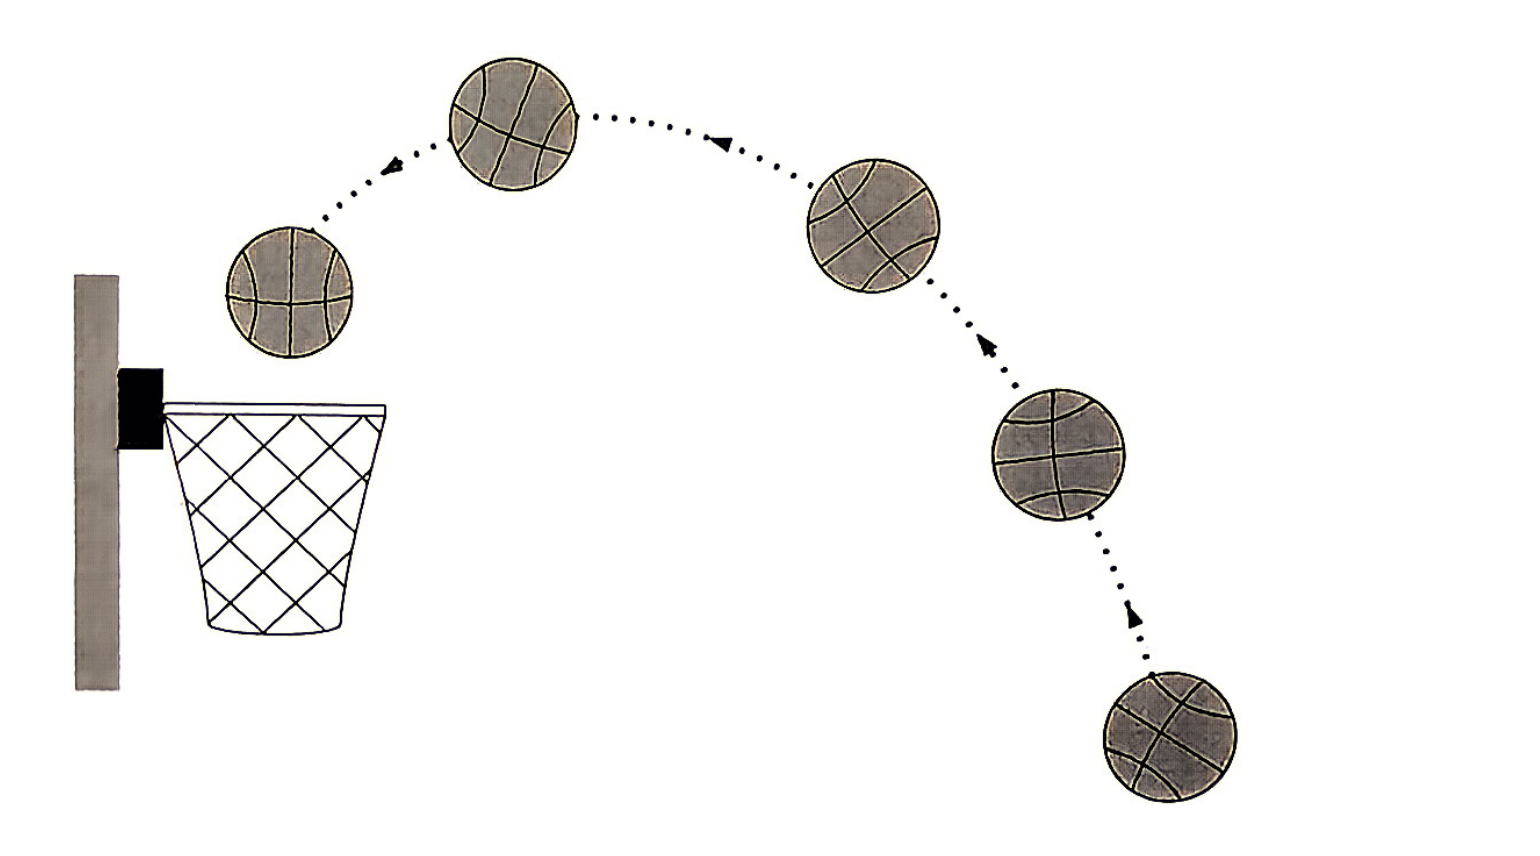
\includegraphics[width=0.72\linewidth]{figures/fig_p030_1.png}
  \caption*{图 2.1\quad 篮球的运动轨迹（原书 p.22, Figure 2.1；PDF p.30）}
\end{figure}

18 世纪，数学家已能把球的轨迹描述为欧氏空间中一条端点固定的曲线。具体而言，在 $\R^2$ 中可把轨迹与速度写成
\[
  \gamma(t)=(q_1(t),q_2(t))\in\R^2,\qquad
  \dot\gamma(t)=(\dot q_1(t),\dot q_2(t))\in\R^2 .
\]
% >>> p031
这里 $\gamma(t)$ 满足边界条件 $\gamma(0)=I$、$\gamma(1)=E$，其中 $I,E\in\R^2$ 为某些固定点。这样就得到一个点对 $(\gamma(t),\dot\gamma(t))\in T\R^2$，其中 $\dot\gamma(t)$ 是点 $\gamma(t)$ 处的切向量。革命性的想法是：对每条连接 $I$ 与 $E$ 的路径赋予一个数值，于是这条抛物轨迹会在所有这些路径中表现为「最优」的一条。为描述这一点，我们将使用物理学中的\textbf{作用量}（action）这一术语。

\begin{wdefn}{2.1.1}
给定光滑函数 $L:T\R^2\to\R$，对路径 $\gamma=\{\gamma(t)\}_{t\in[0,1]}$，定义其\textbf{作用量}为
\begin{equation*}
  \mathcal{A}_L(\gamma):=\int_0^1L(\gamma(t),\dot\gamma(t))\,\dd t .
\end{equation*}
\end{wdefn}
% [Tutor Note: 作用量 $\mathcal{A}_L$ 是定义在路径空间（连接定点 $I,E$ 的 $C^1$ 路径全体）上的泛函，而非定义在 $T\R^2$ 上；$L$ 的变量是位置与速度 $(q,v)\in T\R^2$，积分则沿 $\gamma$ 进行。此处 $\mathcal{A}$ 用花体，注意与 Area 算子 $\Area$ 区分。]

关于作用量 $\mathcal{A}_L$ 有一个自然的问题。

\begin{wque}{2.1.1}
在所有这些端点固定的路径 $\gamma=\{\gamma(t)\}_{t\in[0,1]}$ 中，哪一条使作用量最小？
\end{wque}

如同标准微积分中那样，函数（泛函）的极小点的必要条件必为临界点。应用于作用量 $\mathcal{A}_L$，其临界点可由如下方程描述：
\begin{equation}
  \left.\frac{\dd}{\dd\varepsilon}\mathcal{A}_L(\gamma_\varepsilon)\right|_{\varepsilon=0}=0,
  \tag{2.1}
\end{equation}
其中 $\gamma_\varepsilon(t)=(q_1(t)+\varepsilon c_1(t),q_2(t)+\varepsilon c_2(t))$，$\varepsilon>0$ 充分小，而 $c_i(t)$ 是满足 $c_i(0)=c_i(1)=0$（$i=1,2$）的光滑函数。由定义 2.1.1，方程 (2.1) 等价于
\[
  \left.\frac{\dd}{\dd\varepsilon}\int_0^1L(\gamma_\varepsilon(t),\dot\gamma_\varepsilon(t))\,\dd t
  \right|_{\varepsilon=0}=0 .
\]
% [Tutor Note: 变分路径 $\gamma_\varepsilon$ 必须保持端点不动，故要求 $c_i(0)=c_i(1)=0$；若端点也随 $\varepsilon$ 变化，则下方分部积分会产生额外的边界项。这里 $\left.\frac{\dd}{\dd\varepsilon}\right|_{\varepsilon=0}$ 就是泛函 $\mathcal{A}_L$ 在 $\gamma$ 处沿方向 $c=(c_1,c_2)$ 的 Gâteaux 导数。]
显式地在坐标 $(q,v)\in T\R^2$ 中把它写开：
\[
  \sum_{i=1}^2\int_0^1\left(\frac{\partial L}{\partial q_i}c_i(t)
  +\frac{\partial L}{\partial v_i}\dot c_i(t)\right)(\gamma_\varepsilon(t),\dot\gamma_\varepsilon(t))\,\dd t
  \bigg|_{\varepsilon=0}=0 .
\]
为分离出含 $c_i(t)$ 的项，作分部积分，得
\[
  \sum_{i=1}^2\int_0^1\left(\frac{\partial L}{\partial q_i}c_i(t)
  -\frac{\dd}{\dd t}\frac{\partial L}{\partial v_i}c_i(t)\right)(\gamma_\varepsilon(t),\dot\gamma_\varepsilon(t))\,\dd t
  \bigg|_{\varepsilon=0}=0 .
\]
这等价于如下方程
\[
  \sum_{i=1}^2\int_0^1\left(\frac{\partial L}{\partial q_i}
  -\frac{\dd}{\dd t}\frac{\partial L}{\partial v_i}\right)(\gamma_\varepsilon(t),\dot\gamma_\varepsilon(t))
  \cdot c_i(t)\,\dd t\bigg|_{\varepsilon=0}=0 .
\]
% >>> p032
由于最后这个等式对任意 $c_i(t)$ 都成立，它表明作为 $\mathcal{A}_L$ 的临界点的路径 $\{\gamma(t)\}_{t\in[0,1]}$ 满足如下方程组：
\begin{equation}
  \frac{\partial L}{\partial q_i}(\gamma(t),\dot\gamma(t))
  =\frac{\dd}{\dd t}\frac{\partial L}{\partial v_i}(\gamma(t),\dot\gamma(t))
  \qquad\text{对 } i=1,2 .
  \tag{2.2}
\end{equation}
这组二阶微分方程称为 \textbf{Euler--Lagrange 方程}。反过来，下面给出路径 $\{\gamma(t)\}_{t\in[0,1]}$ 成为作用量 $\mathcal{A}_L$ 的（局部）极小点的一个充分条件。
% [Tutor Note: 从「对任意 $c_i(t)$ 成立」推出被积函数恒为零，依据的是变分法基本引理（du Bois-Reymond 引理）：若连续函数与一切紧支光滑函数的内积为零，则该函数恒为零。这也解释了为何需要 $L$ 光滑、$\gamma$ 至少 $C^2$。此外，「临界点」只是极小点的必要条件而非充分条件——抛体轨迹虽为临界点，但作用量沿某些方向也可能是极大或鞍点。]

\whead{事实}{2.1.1}（[39] 中的定理 19.3）\quad 设定义 2.1.1 中给定的函数 $L:T\R^2\to\R$ 满足如下附加条件：对任意 $q\in\R^2$，$L(q,\cdot)$ 严格凸，即矩阵
\[
  \left(\frac{\partial^2L(q,\cdot)}{\partial v_i\partial v_j}\right)
\]
正定。若路径 $\{\gamma(t)\}_{t\in[0,1]}$ 满足 Euler--Lagrange 方程，则它是作用量 $\mathcal{A}_L$ 的局部极小点。
% [Tutor Note: 严格凸性正是把「临界点」升级为「极小点」的关键：沿任意固定端点的变分 $c$，作用量的二阶变分等于 $\int_0^1\sum_{i,j}\frac{\partial^2L}{\partial v_i\partial v_j}\dot c_i\dot c_j\,\dd t$ 再加一项与 $c$ 无关的项，由 Hessian 正定即得正定；这也是后文 §2.2 中 Legendre 变换可逆（$v\mapsto p=\partial_vL$ 为微分同胚）的同一条件。]

定义 2.1.1 中函数 $L$ 的一个常见取法是所谓的\textbf{拉格朗日量}（Lagrangian）。在经典力学中，拉格朗日量就是动能\emph{减去}势能（而按定义，总能量是动能\emph{加上}势能）。
% [Tutor Note: 术语依据——原文名词 Lagrangian 指拉格朗日函数（量），本译本统一作「拉格朗日量」；形容词用法（Lagrangian submanifold）仍作「拉格朗日子流形」，二者不可混同。]

\begin{wexam}{2.1.1}
（拉格朗日量）在 $\R^2$ 中，取
\begin{equation}
  L(q,v)=\frac12m|v(t)|^2-mgq_2(t),
  \tag{2.3}
\end{equation}
其中 $q=(q_1(t),q_2(t))\in\R^2$，而 $v=(v_1(t),v_2(t))\in T_q\R^2$ 为速度。这里 $\frac12m|v|^2$ 是动能，$mgq_2$ 代表势能。对路径 $\{\gamma(t)\}_{t\in[0,1]}$ 与 (2.3) 中的拉格朗日量 $L$，Euler--Lagrange 方程计算如下：
\[
  \begin{cases}
    0=\dfrac{\dd}{\dd t}mv_1(t)(\gamma(t),\dot\gamma(t))=m\ddot q_1(t)\\[2mm]
    mg=\dfrac{\dd}{\dd t}mv_2(t)(\gamma(t),\dot\gamma(t))=m\ddot q_2(t)
  \end{cases}
\]
% [Tutor Note: 原文疑误——由 (2.3) 得 $\partial L/\partial q_2=-mg$，故第二式左端应为 $-mg$（即 $m\ddot q_2=-mg$），而非 $mg$；否则与下文「$q_2$ 为抛物函数」及抛物线开口向下矛盾。译文保留原文写法，详见 review_ch02.md。另注：原文把 $L(q,v)$ 中的 $v$ 写成 $v(t)$、$q_2$ 写成 $q_2(t)$，是记号混用，$L$ 的自变量应为定点的 $(q,v)$。]
由上述方程可知 $q_1(t)$ 是线性的，而 $q_2(t)$ 是抛物线的（因 $g\neq0$）。于是把 $q_2(t)$ 中的 $t$ 用变量 $q_1$ 替换，$q_2$ 便是关于 $q_1$ 的抛物函数，这说明 $\gamma(t)$ 在 $\R^2$ 中描出一条抛物线。\hfill$//$
\end{wexam}

下面这个例子与流形上的测地线有关。事实上，它给出了推导测地线表达式的一种不同但等价的方式。

\begin{wexam}{2.1.2}
（测地线）在带度量 $g=(g_{ij})_{1\le i,j\le2}$ 的 Riemann 曲面 $(M^2,g)$ 上，考虑局部定义的函数 $L:TM\to\R$：
\[
  L(q,v)=\frac12\sum_{1\le i,j\le2}g_{ij}(q)v_i(t)v_j(t).
\]
% >>> p033
注意这里 $L$ 满足事实 2.1.1 中的「严格凸」条件，因为 Riemann 度量 $g$ 给出的矩阵 $(g_{ij}(q))_{1\le i,j\le2}$ 对任意 $q\in M$ 都正定。下面我们将证明，作用量 $\mathcal{A}_L$ 的极小点等价于 $(M^2,g)$ 上的测地线。

由事实 2.1.1，只需算出此情形下的 Euler--Lagrange 方程，并确认它们等价于 $(M^2,g)$ 的测地线方程
\[
  \ddot q_k+\sum_{1\le i,j\le2}\Gamma^k_{ij}\dot q_i\dot q_j=0
  \qquad\text{对 } k=1,2 .
\]
这里记号 $\Gamma^k_{ij}$ 表示 $\Gamma^k_{ij}=\sum_{i=1}^2g^{kl}\Gamma_{lij}$，其中
\[
  (g^{ij})=(g_{ij})^{-1}
  \qquad\text{以及}\qquad
  \Gamma_{lij}:=\frac12\left(\frac{\partial g_{il}}{\partial q_j}
  +\frac{\partial g_{jl}}{\partial q_i}-\frac{\partial g_{ij}}{\partial q_l}\right).
\]
% [Tutor Note: 原文疑误——上式右端的和式指标应为 $l$（$\Gamma^k_{ij}=\sum_{l=1}^2g^{kl}\Gamma_{lij}$），原文写成对 $i$ 求和，与左端的自由指标 $k$ 及被求和式 $\Gamma_{lij}$ 的 Einstein 约定均不相容。译文保留原文写法，详见 review_ch02.md。另请注意 $(g^{ij})$ 是 $(g_{ij})$ 的逆矩阵，此处 $g^{ij}$ 并非「度量的分量」而是「逆度量的分量」。]
由 (2.2)，
\[
  g_{ik}\ddot q_i+\frac12\left(\frac{\partial g_{ik}}{\partial q_j}
  +\frac{\partial g_{jk}}{\partial q_i}-\frac{\partial g_{ij}}{\partial q_k}\right)\dot q_i\dot q_j=0
  \qquad\text{对 } k=1,2,
\]
即
\[
  g_{ik}\ddot q_i+\Gamma_{kij}\dot q_i\dot q_j=0\qquad\text{对 } k=1,2 .
\]
把 $k=1$ 与 $k=2$ 的两个方程合在一起，可重写为矩阵形式：
\[
  (g_{ij})\begin{pmatrix}\ddot q_1\\ \ddot q_2\end{pmatrix}
  =-\begin{pmatrix}\Gamma_{1ij}\dot q_i\dot q_j\\ \Gamma_{2ij}\dot q_i\dot q_j\end{pmatrix}.
\]
于是得到
\[
  \begin{pmatrix}\ddot q_1\\ \ddot q_2\end{pmatrix}
  =-(g^{ij})\begin{pmatrix}\Gamma_{1ij}\dot q_i\dot q_j\\ \Gamma_{2ij}\dot q_i\dot q_j\end{pmatrix}
  =-\begin{pmatrix}\sum_{1\le i,j\le2}\Gamma^1_{ij}\dot q_i\dot q_j\\[1mm]
  \sum_{1\le i,j\le2}\Gamma^2_{ij}\dot q_i\dot q_j\end{pmatrix},
\]
恰与测地线方程等价，证毕。\hfill$//$
\end{wexam}
% [Tutor Note: 此处所有 $g_{ik}\ddot q_i$、$\Gamma_{kij}\dot q_i\dot q_j$ 都按 Einstein 约定对重复指标 $i,j$ 求和；$k$ 是自由指标。$\Gamma_{kij}=\frac12(\partial_jg_{ik}+\partial_ig_{jk}-\partial_kg_{ij})$ 是第一类 Christoffel 符号，而 $\Gamma^k_{ij}=g^{kl}\Gamma_{lij}$ 是第二类。矩阵式左端 $(g_{ij})(\ddot q_1,\ddot q_2)^{\mathrm T}$ 的第 $k$ 个分量正是 $g_{ki}\ddot q_i$。]
